% Adapted from the repository's original state-ownership diagram.
\begin{figure}[tbp]
\centering
\resizebox{\linewidth}{!}{%
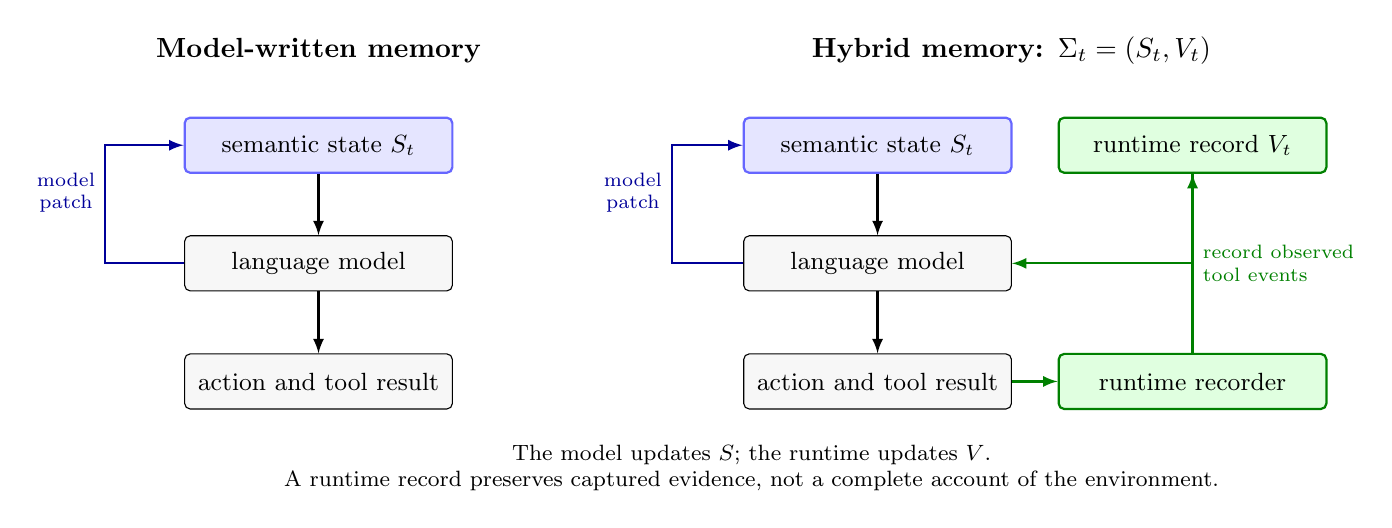
\begin{tikzpicture}[
font=\small,
box/.style={draw,rounded corners=2pt,minimum width=3.4cm,minimum height=.7cm,align=center,inner sep=3pt},
state/.style={box,fill=blue!10,draw=blue!60,thick},
record/.style={box,fill=green!12,draw=green!50!black,thick},
plain/.style={box,fill=black!3},
arr/.style={-latex,thick}]
\node[font=\bfseries] at (0,3.5) {Model-written memory};
\node[state] (s1) at (0,2.3) {semantic state $S_t$};
\node[plain] (m1) at (0,.8) {language model};
\node[plain] (a1) at (0,-.7) {action and tool result};
\draw[arr] (s1)--(m1);
\draw[arr] (m1)--(a1);
\draw[arr,blue!60!black] (m1.west)--++(-1,0)|-(s1.west)
node[pos=.3,left,font=\scriptsize,align=center]{model\\patch};
\begin{scope}[xshift=7.1cm]
\node[font=\bfseries] at (1.7,3.5) {Hybrid memory: $\Sigma_t=(S_t,V_t)$};
\node[state] (s2) at (0,2.3) {semantic state $S_t$};
\node[record] (v2) at (4,2.3) {runtime record $V_t$};
\node[plain] (m2) at (0,.8) {language model};
\node[plain] (a2) at (0,-.7) {action and tool result};
\node[record] (rec) at (4,-.7) {runtime recorder};
\draw[arr] (s2)--(m2);
\draw[arr,green!50!black] (v2.south)|-(m2.east);
\draw[arr] (m2)--(a2);
\draw[arr,blue!60!black] (m2.west)--++(-.9,0)|-(s2.west)
node[pos=.3,left,font=\scriptsize,align=center]{model\\patch};
\draw[arr,green!50!black] (a2)--(rec);
\draw[arr,green!50!black] (rec)--(v2)
node[midway,right,font=\scriptsize,align=left]{record observed\\tool events};
\end{scope}
\node[font=\footnotesize,align=center] at (5.5,-1.8)
{The model updates $S$; the runtime updates $V$.\\A runtime record preserves captured evidence, not a complete account of the environment.};
\end{tikzpicture}}
\caption{State ownership. Hybrid memory retains model-written semantic content and adds runtime-derived records. Recording an event does not establish that an extracted interpretation is correct or that all relevant events were captured.}
\label{fig:runtime-written}
\end{figure}
